\documentclass{standalone}
\usepackage{tikz}
\usetikzlibrary[automata,positioning,arrows]
\tikzset{node distance=2.5cm,
         every state/.style={
             semithick,
             fill=gray!10
         },
         initial text={},
         double distance=2pt,
         every edge/.style={
             draw,
             ->,>=stealth',
             auto,
             semithick
         }}
\let\epsilon\varepsilon

\begin{document}

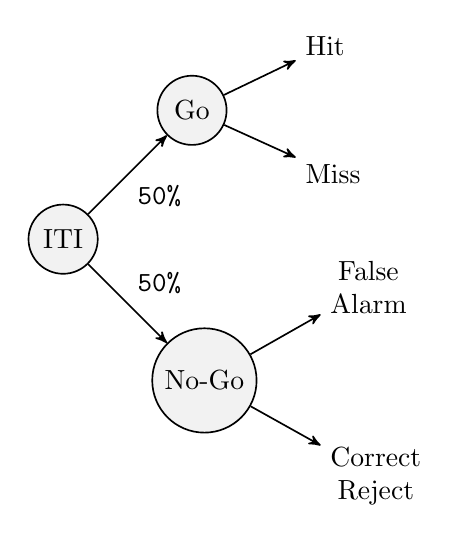
\begin{tikzpicture}
  \node[state] (iti) {ITI};
  \node[state, above right=1cm and 1cm of iti] (go) {Go};
  \node[state, below right=1cm and 1cm of iti] (nogo) {No-Go};
  \node[above right=0.25cm and 1cm of go] (hit) {Hit};
  \node[below right=0.25cm and 1cm of go] (miss) {Miss};
  \node[above right=0.25cm and 1cm of nogo, align=center] (false-alarm) {False\\Alarm};
  \node[below right=0.25cm and 1cm of nogo, align=center] (correct-reject) {Correct\\Reject};
  \draw (iti) edge node[below right] {\tt 50\%} (go);
  \draw (iti) edge node {\tt 50\%} (nogo);
  \draw (go) edge (hit);
  \draw (go) edge (miss);
  \draw (nogo) edge (false-alarm);
  \draw (nogo) edge (correct-reject);
\end{tikzpicture}

\end{document}